
In order to evaluate the proposed approach of axiom weakening, specifically for its application in the context of automatic repair of ontologies, we need a way to compare the quality of different possible repairs. As has already been discussed in \cite{troquard2018repairing}, the problem of deciding which of two possible repaired ontologies $\Omc_1$ or $\Omc_2$ is preferable is not generally well-defined. As such, this thesis will use the same measure defined for the experimental evaluation in \cite{troquard2018repairing}. The main idea is to use the size of the \emph{inferred class hierarchy} to evaluate the amount of ``information'' a repair can retain.

\begin{definition}\label{def:inf}
  The \emph{inferred class hierarchy} of an ontology $\Omc$ is given by
  \begin{align*}
    \Inf(\Omc) = \{ A \sqsubseteq B \mid A, B \in N_C \text{ and } A \sqsubseteq_\Omc B \} \enspace.
  \end{align*}
\end{definition}

To compare the relative amount of ``information'' between two ontologies, we compare them based on their differences in the inferred class hierarchy. We use for this purpose the \emph{inferable information content} (IIC) as defined in \cite{troquard2018repairing}.

\begin{definition}\label{def:iic}
  The \emph{inferable information content} of an ontology $\Omc_1$ with respect to another ontology $\Omc_2$ is given by
  \begin{align*}
    \qual(\Omc_1, \Omc_2) = \frac{| \Inf(\Omc_1) \setminus \Inf(\Omc_2) |}{|\Inf(\Omc_1) \setminus \Inf(\Omc_2)| + |\Inf(\Omc_2) \setminus \Inf(\Omc_1)|} \enspace,
  \end{align*}
  where $|X|$ is the cardinality of the set $X$.
\end{definition}

The IIC of an ontology $\Omc_1$ with respect to a second ontology $\Omc_2$, written $\qual(\Omc_1, \Omc_2)$, is a number between $0$ and $1$. A value closer to $1$ indicates that $\Omc_1$ contains more ``information'' than $\Omc_2$, while a value towards $0$ indicates the opposite. Inferred hierarchy axioms common to both ontologies do not influence the results, and if $\Omc_2$ is entailed by $\Omc_1$, then the IIC of $\Omc_1$ with respect to $\Omc_2$ is always $1$. If both $\Omc_1$ and $\Omc_2$ have some inferences that are not shared by the other ontology, the IIC will be strictly between $0$ and $1$. Note that if the cardinality of the inferred class hierarchy is larger for one ontology, then it will also be the one preferred by the IIC. Some weaknesses of this measure when it comes to evaluating repairs, like the fact that only atomic concepts are considered, have already been discussed in \cite{troquard2018repairing}. For the case of repairing \SROIQ ontologies, this is even more relevant, since the role hierarchy is entirely ignored.

The evaluation starts by first making the ontologies inconsistent. This has been achieved by repeatedly adding axioms to the ontology until it was no longer consistent. The newly added axioms were generated by strengthening randomly selected axioms of the ontology. Axioms are strengthened by applying an axiom strengthening operator, that is equivalent to the axiom weakening operator in \cref{def:weaken}, except for swapping the generalization and specialization operators and not using $\bot \sqsubseteq \top$ to remove the axiom. An axiom $\alpha'$ is stronger than another axiom $\alpha$ with respect to the ontology $\Omc$ if $\alpha' \models_\Omc \alpha$. Note that this is only a useful characterization if $\alpha \not\in \Omc$. It was ensured that the added axioms on their own were not inconsistent. After making the ontology inconsistent, it was repaired using different automatic repair algorithms. Each inconsistent ontology was repaired once with the repair algorithm using the axiom weakening operator presented in \cref{algo:repair-weaken} and once using \cref{algo:repair-remove}. As can be seen in \cref{ex:alc-weakening}, choosing a maximal consistent subset can sometimes lead to less information loss than using the weakening based algorithm. To experimentally evaluate how good weakening performs against the maximal consistent subset based repair on average, the repair was also performed by selecting a randomly sampled maximal consistent subset.

\begin{algorithm}[ht]
  \begin{algorithmic}
    \While{$\Omc$ is inconsistent}
      \State $\phi_\textnormal{bad} \gets \textsc{FindBadAxiom}(\Omc)$
      \State $\Omc \gets \Omc \setminus \{\phi_\textnormal{bad}\}$
    \EndWhile
    \State Return $\Omc$
  \end{algorithmic}
  \caption{$\textsc{RepairOntologyRemove}(\Omc)$}
  \label{algo:repair-remove}
\end{algorithm}

This process, both making the ontology inconsistent and repairing it, was repeated one hundred times for each ontology, and the IIC was computed between the results obtained using the different repair methods. The evaluation was performed using a randomly sampled maximal consistent subset as the reference ontology and by randomly sampling $16$ minimal inconsistent subsets during the selection of bad axioms in $\textsc{FindBadAxiom}$. To obtain comparable results, both $\textsc{RepairOntologyRemove}$ and $\textsc{RepairOntologyWeakening}$ use the same implementation of $\textsc{FindBadAxiom}$. While the utilized OWL 2 DL reasoners are all highly optimized, they exhibit undesirable performance in some edge cases. Mostly they are fast to perform reasoning tasks like checking for consistency or entailment in the selected ontologies. However, when performance pitfalls are encountered, they may require significantly more time, making the computations required for repair unreasonably slow. For this reason, a timeout of 5 minutes was placed on the repairs execution and the outputs of runs that did not complete within this time limit were discarded and replaced by new runs. The results of these experiments are listed in \cref{table:results} and shown in \cref{fig:results-remove} and \cref{fig:results-mcs}.

\begin{table}[ht]
  \scriptsize
  \centering
  \begin{tabular}{|l|cc@{ }c|}
    \cline{2-4}
    \multicolumn{1}{l|}{} & IIC w.r.t. removal & \multicolumn{2}{c|}{IIC w.r.t. maximal consistent subset} \\
    \hline
    admin & 0.56 [0.51, 0.60] & 0.39 [0.33, 0.45] & (0.51 [0.45, 0.57]) \\
    ahso & 0.57 [0.52, 0.62] & 0.52 [0.47, 0.56] & (0.64 [0.59, 0.69]) \\
    cdao & 0.54 [0.49, 0.61] & 0.51 [0.44, 0.57] & (0.55 [0.48, 0.61]) \\
    cdpeo & 0.50 [0.47, 0.53] & 0.25 [0.20, 0.30] & (0.39 [0.33, 0.45]) \\
    covid19-ibo & 0.71 [0.67, 0.75] & 0.62 [0.58, 0.66] & (0.72 [0.68, 0.76]) \\
    ecp & 0.75 [0.70, 0.80] & 0.36 [0.30, 0.42] & (0.50 [0.44, 0.56]) \\
    emo & 0.68 [0.63, 0.72] & 0.61 [0.56, 0.65] & (0.73 [0.68, 0.77]) \\
    evi & 0.51 [0.46, 0.55] & 0.58 [0.53, 0.63] & (0.71 [0.66, 0.75]) \\
    falls & 0.75 [0.70, 0.81] & 0.50 [0.44, 0.57] & (0.60 [0.54, 0.66]) \\
    fo & 0.53 [0.48, 0.58] & 0.68 [0.63, 0.73] & (0.67 [0.62, 0.73]) \\
    gbm & 0.59 [0.54, 0.64] & 0.54 [0.49, 0.59] & (0.68 [0.63, 0.73]) \\
    gfvo & 0.53 [0.47, 0.58] & 0.54 [0.49, 0.59] & (0.71 [0.67, 0.75]) \\
    koro & 0.53 [0.48, 0.58] & 0.38 [0.32, 0.43] & (0.53 [0.47, 0.59]) \\
    lico & 0.53 [0.48, 0.59] & 0.51 [0.46, 0.57] & (0.63 [0.58, 0.68]) \\
    mamo & 0.55 [0.49, 0.61] & 0.64 [0.58, 0.69] & (0.72 [0.66, 0.77]) \\
    mpio & 0.69 [0.65, 0.74] & 0.70 [0.66, 0.75] & (0.70 [0.65, 0.74]) \\
    pizza & 0.56 [0.51, 0.62] & 0.57 [0.51, 0.63] & (0.63 [0.58, 0.69]) \\
    provo & 0.51 [0.47, 0.56] & 0.55 [0.51, 0.60] & (0.64 [0.60, 0.69]) \\
    qudt & 0.96 [0.93, 0.98] & 0.47 [0.40, 0.53] & (0.56 [0.49, 0.62]) \\
    trans & 0.56 [0.51, 0.61] & 0.41 [0.35, 0.47] & (0.51 [0.45, 0.57]) \\
    triage & 0.51 [0.46, 0.56] & 0.52 [0.47, 0.57] & (0.63 [0.57, 0.68]) \\
    vio & 0.48 [0.41, 0.54] & 0.50 [0.44, 0.57] & (0.57 [0.51, 0.63]) \\
    \hline
    Overall & 0.60 [0.58, 0.61] & 0.52 [0.50, 0.53] & (0.61 [0.60, 0.63]) \\
    \hline
  \end{tabular}
  \caption{Results of the evaluation. IIC is given as mean and 95\% confidence interval in brackets. The values in parentheses are for weakening that does not weaken the axioms in the maximal consistent subset chosen as reference ontology.}
  \label{table:results}
\end{table}

\begin{figure}[ht]
  \centering
  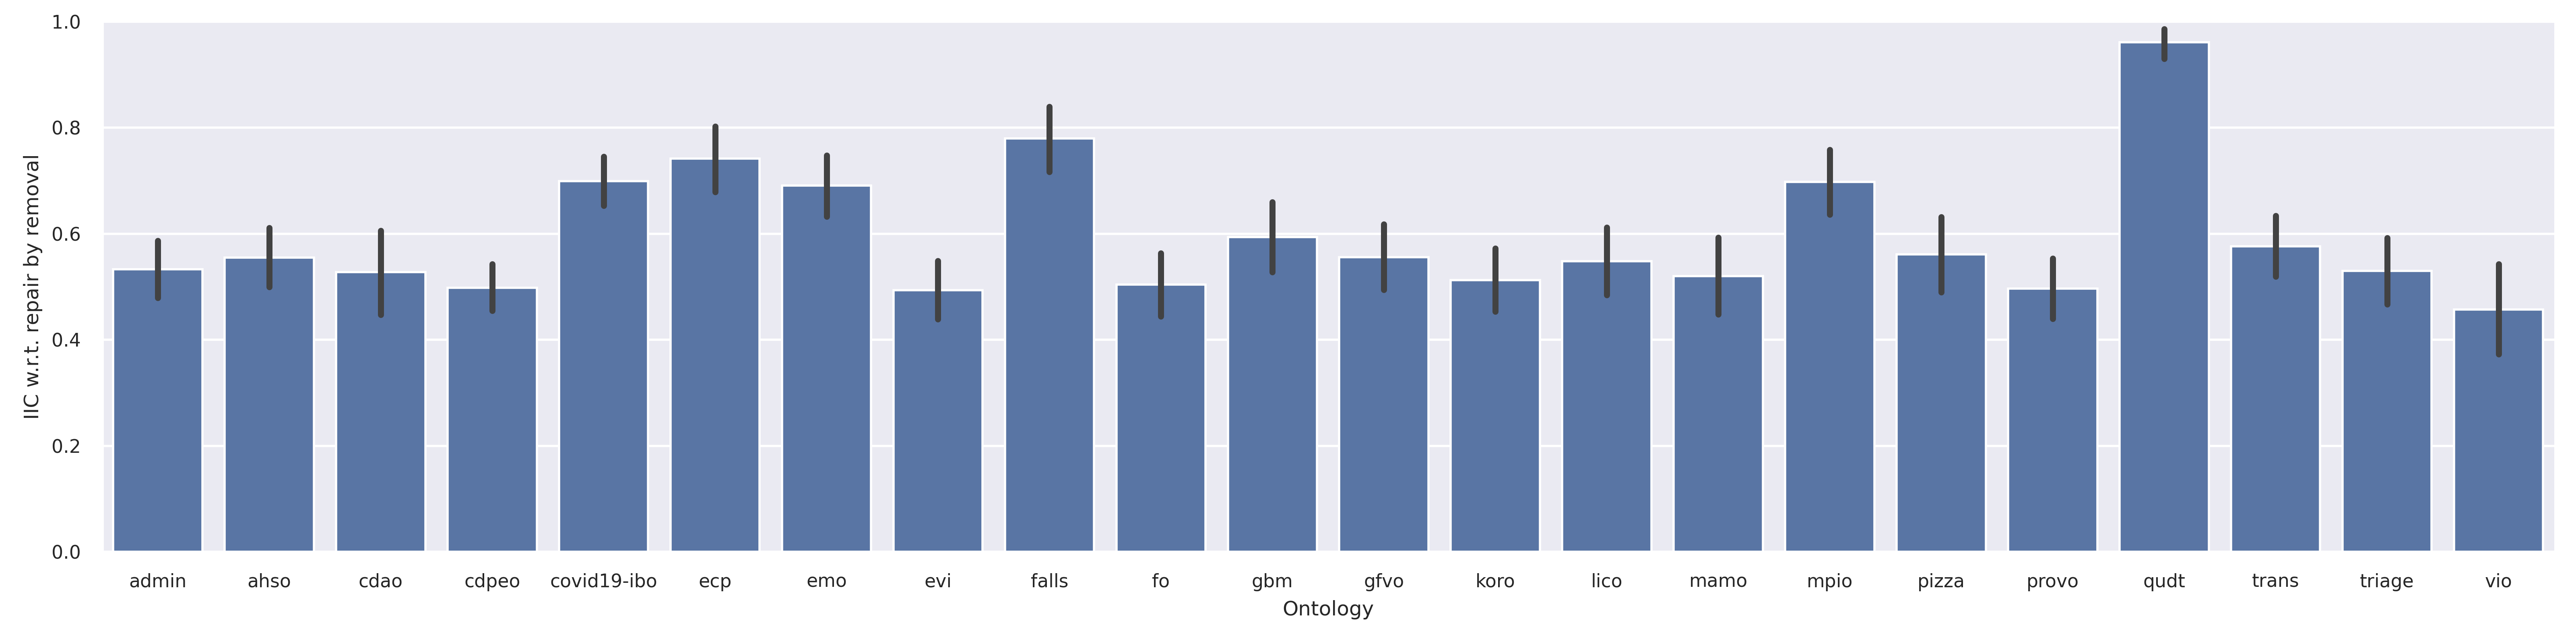
\includegraphics[width=\textwidth]{resources/iic-remove-ontology-bar.png}
  \caption{Mean IIC with respect to repair via removal per ontology. The error bars show the 95\% confidence interval.}
  \label{fig:results-remove}
\end{figure}

The results of the evaluation suggest that the repair by weakening is on average about as good or better than the repair by removal. While this supports the conclusion in \cite{troquard2018repairing} that axiom weakening is able to retain more information than removal, the observed advantage was smaller than what has been observed in \cite{troquard2018repairing}.

\begin{figure}[ht]
  \centering
  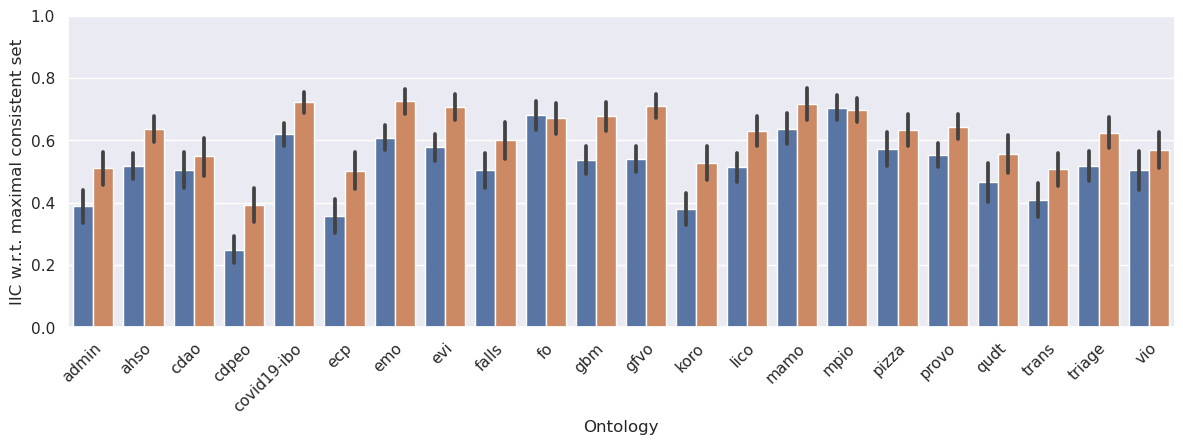
\includegraphics[width=\textwidth]{resources/iic-both-mcs-ontology-bar.png}
  \caption{Mean IIC with respect to a random maximal consistent subset. The error bars show the 95\% confidence interval. The orange bars used a variation of the repair by weakening, where axioms in the reference ontology are never weakened.}
  \label{fig:results-mcs}
\end{figure}

In contrast, it can be seen that the repair using weakening is not always better than choosing a random maximal consistent subset. There are ontologies for which the repair by weakening is on average significantly worse when comparing using IIC. This is, however, a somewhat unequal comparison. We have seen in \cref{ex:alc-weakening} also a situation in which weakening performs worse when it comes to preserving information compared to choosing a maximally consistent subset. A more equal comparison, yet still not perfect since the maximal consistent subset for the reference ontology is not chosen uniformly at random, would be to a repair algorithm that starts with the reference ontology and uses axiom weakening to add more information from the remaining axioms. This has been implemented and evaluated, and the results can be seen as the orange bars in \cref{fig:results-mcs}. Still, this result suggests that the heuristic used for selecting bad axioms is not reliable for preserving information, at least when measured using IIC. It has not been closely studied what causes the repair by weakening to significantly lose for some ontologies while being clearly preferred in others. Interestingly, there are also some cases in which the weakening based repair performs better against a random maximal consistent subset than against the repair by removal.

To overcome some weaknesses of the IIC, especially that it does not account for subsumptions between roles or complex concept expressions, tests were also carried out using an extended version of the inferred class hierarchy and IIC, adding to it subsumptions between subconcepts and roles.

\begin{definition}
  The \emph{extended inferred class hierarchy} of an ontology $\Omc$ is given by
  \begin{align*}
    \Inf^+(\Omc) ={} & \{ C \sqsubseteq D \mid C, D \in \sub(\Omc) \text{ and } C \sqsubseteq_\Omc D \} \\
    & \cup \{ R \sqsubseteq S \mid R, S \in \Lmc(N_R) \text{ and } R \sqsubseteq_\Omc S \} \enspace.
  \end{align*}
  The \emph{extended inferable information content} (IIC$^+$) of an ontology $\Omc_1$ with respect to another ontology $\Omc_2$ is given by
  \begin{align*}
    \qual^+(\Omc_1, \Omc_2) = \frac{| \Inf^+(\Omc_1) \setminus \Inf^+(\Omc_2) |}{|\Inf^+(\Omc_1) \setminus \Inf^+(\Omc_2)| + |\Inf^+(\Omc_2) \setminus \Inf^+(\Omc_1)|} \enspace,
  \end{align*}
\end{definition}

Of course, this new measure still only captures a small part of all consequences, but it should provide more accurate results when it comes to information about subconcepts and roles. When evaluating the experiment outcomes, we see that the values produced by IIC and IIC$^+$ are very similar. As may be expected, the repair by weakening is preferred slightly more strongly when using IIC$^+$. \Cref{fig:results-eiic} shows the comparison between IIC and IIC$^+$ for repair using axiom weakening w.r.t. repair by removal. The differences between IIC and IIC$^+$ are somewhat stronger when comparing against the repair using a random maximal consistent subset, but the differences are still not particularly noteworthy.

\begin{figure}[ht]
  \centering
  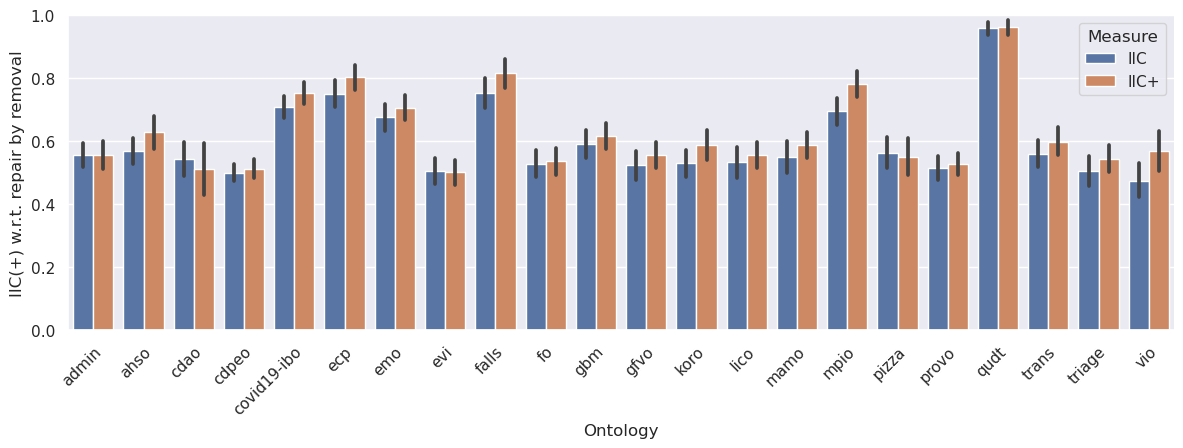
\includegraphics[width=\textwidth]{resources/iic-eiic-ontology-bar.png}
  \caption{Mean IIC and IIC$^+$ with respect to repair by removal per ontology. The error bars show the 95\% confidence interval.}
  \label{fig:results-eiic}
\end{figure}
